% documentclass: article used for scientific journals, short reports, program documentation, etc
% options: fontsize 11, generate document for double sided printing, a4-paper
\documentclass[11pt, twoside, a4paper]{article}

% package for changing page layout
\usepackage{geometry}
\geometry{a4paper, lmargin=30mm, rmargin=20mm, tmargin=30mm, bmargin=20mm}
% set indentation
\setlength{\parindent}{0mm} 

% input encoding for special characters (e.g. ä,ü,ö,ß), only for non english text
% options: utf8 as encoding standard
\usepackage[utf8]{inputenc}
% package for changing used language
% options: german or default: english
\usepackage[german]{babel}

% package for math symbols, functions and environments from ams(american mathematical society)
\usepackage{amsmath}
% package for extended symbols from ams
\usepackage{amssymb}
% package for extended symbols from stmaryrd(st mary road)
%\usepackage{stmaryrd}
% package for managing pictures
\usepackage{graphicx}

% package for some extra fonts
\usepackage{txfonts}
% package for changing color of font and paper
% options: using names of default colors (e.g red, black)
\usepackage[usenames]{color}

% package for converting eps-files to pdf-files and then include them
\usepackage{epstopdf}
% use another program (ps2pdf) for converting
% !!! important: set shell_escape=1 in /etc/texmf/texmf.cnf (Linux) for allowing to use other programs
% !!!			 or use the command line with -shell-escape
\epstopdfDeclareGraphicsRule{.eps}{pdf}{.pdf}{
ps2pdf -dEPSCrop #1 \OutputFile
}

% package for reference to last page (output number of last page)
\usepackage{lastpage}
% package for using header and footer
% options: automate terms of right and left marks
\usepackage[automark]{scrpage2}
% set style for footer and header
\pagestyle{scrheadings}
% clear pagestyle for redefining
\clearscrheadfoot
% set header and footer: use <xx>head/foot[]{Text} (i...inner, o...outer, c...center, o...odd, e...even, l...left, r...right)
\ihead[]{}
\ohead[]{}
\cfoot[]{\pagemark/\pageref{LastPage}}


% begin the document
\begin{document}
	
	\begin{figure}[h]
		\center
		% GNUPLOT: LaTeX picture with Postscript
\begingroup
  \makeatletter
  \providecommand\color[2][]{%
    \GenericError{(gnuplot) \space\space\space\@spaces}{%
      Package color not loaded in conjunction with
      terminal option `colourtext'%
    }{See the gnuplot documentation for explanation.%
    }{Either use 'blacktext' in gnuplot or load the package
      color.sty in LaTeX.}%
    \renewcommand\color[2][]{}%
  }%
  \providecommand\includegraphics[2][]{%
    \GenericError{(gnuplot) \space\space\space\@spaces}{%
      Package graphicx or graphics not loaded%
    }{See the gnuplot documentation for explanation.%
    }{The gnuplot epslatex terminal needs graphicx.sty or graphics.sty.}%
    \renewcommand\includegraphics[2][]{}%
  }%
  \providecommand\rotatebox[2]{#2}%
  \@ifundefined{ifGPcolor}{%
    \newif\ifGPcolor
    \GPcolorfalse
  }{}%
  \@ifundefined{ifGPblacktext}{%
    \newif\ifGPblacktext
    \GPblacktexttrue
  }{}%
  % define a \g@addto@macro without @ in the name:
  \let\gplgaddtomacro\g@addto@macro
  % define empty templates for all commands taking text:
  \gdef\gplbacktext{}%
  \gdef\gplfronttext{}%
  \makeatother
  \ifGPblacktext
    % no textcolor at all
    \def\colorrgb#1{}%
    \def\colorgray#1{}%
  \else
    % gray or color?
    \ifGPcolor
      \def\colorrgb#1{\color[rgb]{#1}}%
      \def\colorgray#1{\color[gray]{#1}}%
      \expandafter\def\csname LTw\endcsname{\color{white}}%
      \expandafter\def\csname LTb\endcsname{\color{black}}%
      \expandafter\def\csname LTa\endcsname{\color{black}}%
      \expandafter\def\csname LT0\endcsname{\color[rgb]{1,0,0}}%
      \expandafter\def\csname LT1\endcsname{\color[rgb]{0,1,0}}%
      \expandafter\def\csname LT2\endcsname{\color[rgb]{0,0,1}}%
      \expandafter\def\csname LT3\endcsname{\color[rgb]{1,0,1}}%
      \expandafter\def\csname LT4\endcsname{\color[rgb]{0,1,1}}%
      \expandafter\def\csname LT5\endcsname{\color[rgb]{1,1,0}}%
      \expandafter\def\csname LT6\endcsname{\color[rgb]{0,0,0}}%
      \expandafter\def\csname LT7\endcsname{\color[rgb]{1,0.3,0}}%
      \expandafter\def\csname LT8\endcsname{\color[rgb]{0.5,0.5,0.5}}%
    \else
      % gray
      \def\colorrgb#1{\color{black}}%
      \def\colorgray#1{\color[gray]{#1}}%
      \expandafter\def\csname LTw\endcsname{\color{white}}%
      \expandafter\def\csname LTb\endcsname{\color{black}}%
      \expandafter\def\csname LTa\endcsname{\color{black}}%
      \expandafter\def\csname LT0\endcsname{\color{black}}%
      \expandafter\def\csname LT1\endcsname{\color{black}}%
      \expandafter\def\csname LT2\endcsname{\color{black}}%
      \expandafter\def\csname LT3\endcsname{\color{black}}%
      \expandafter\def\csname LT4\endcsname{\color{black}}%
      \expandafter\def\csname LT5\endcsname{\color{black}}%
      \expandafter\def\csname LT6\endcsname{\color{black}}%
      \expandafter\def\csname LT7\endcsname{\color{black}}%
      \expandafter\def\csname LT8\endcsname{\color{black}}%
    \fi
  \fi
  \setlength{\unitlength}{0.0500bp}%
  \begin{picture}(8502.00,5102.00)%
    \gplgaddtomacro\gplbacktext{%
      \csname LTb\endcsname%
      \put(814,704){\makebox(0,0)[r]{\strut{}0.0}}%
      \put(814,1279){\makebox(0,0)[r]{\strut{}1.0}}%
      \put(814,1854){\makebox(0,0)[r]{\strut{}2.0}}%
      \put(814,2429){\makebox(0,0)[r]{\strut{}3.0}}%
      \put(814,3004){\makebox(0,0)[r]{\strut{}4.0}}%
      \put(814,3579){\makebox(0,0)[r]{\strut{}5.0}}%
      \put(814,4154){\makebox(0,0)[r]{\strut{}6.0}}%
      \put(946,484){\makebox(0,0){\strut{}0.0}}%
      \put(1741,484){\makebox(0,0){\strut{}0.5}}%
      \put(2537,484){\makebox(0,0){\strut{}1.0}}%
      \put(3332,484){\makebox(0,0){\strut{}1.5}}%
      \put(4128,484){\makebox(0,0){\strut{}2.0}}%
      \put(4923,484){\makebox(0,0){\strut{}2.5}}%
      \put(5719,484){\makebox(0,0){\strut{}3.0}}%
      \put(6514,484){\makebox(0,0){\strut{}3.5}}%
      \put(7310,484){\makebox(0,0){\strut{}4.0}}%
      \put(8105,484){\makebox(0,0){\strut{}4.5}}%
      \put(176,2572){\rotatebox{-270}{\makebox(0,0){\strut{}$f_N \ [Hz]$}}}%
      \put(4525,154){\makebox(0,0){\strut{}$f_K \ [Hz]$}}%
      \put(4525,4771){\makebox(0,0){\strut{}Nutation in Abhängigkeit der Kreiselfrequenz $f_N(f_K)$}}%
      \put(1344,3579){\makebox(0,0)[l]{\strut{}$a\pm \Delta a = 1.513 \pm 0.017 $}}%
    }%
    \gplgaddtomacro\gplfronttext{%
      \csname LTb\endcsname%
      \put(2266,4268){\makebox(0,0)[r]{\strut{}Messwerte}}%
      \csname LTb\endcsname%
      \put(2266,4048){\makebox(0,0)[r]{\strut{}$f(x) = ax$}}%
    }%
    \gplbacktext
    \put(0,0){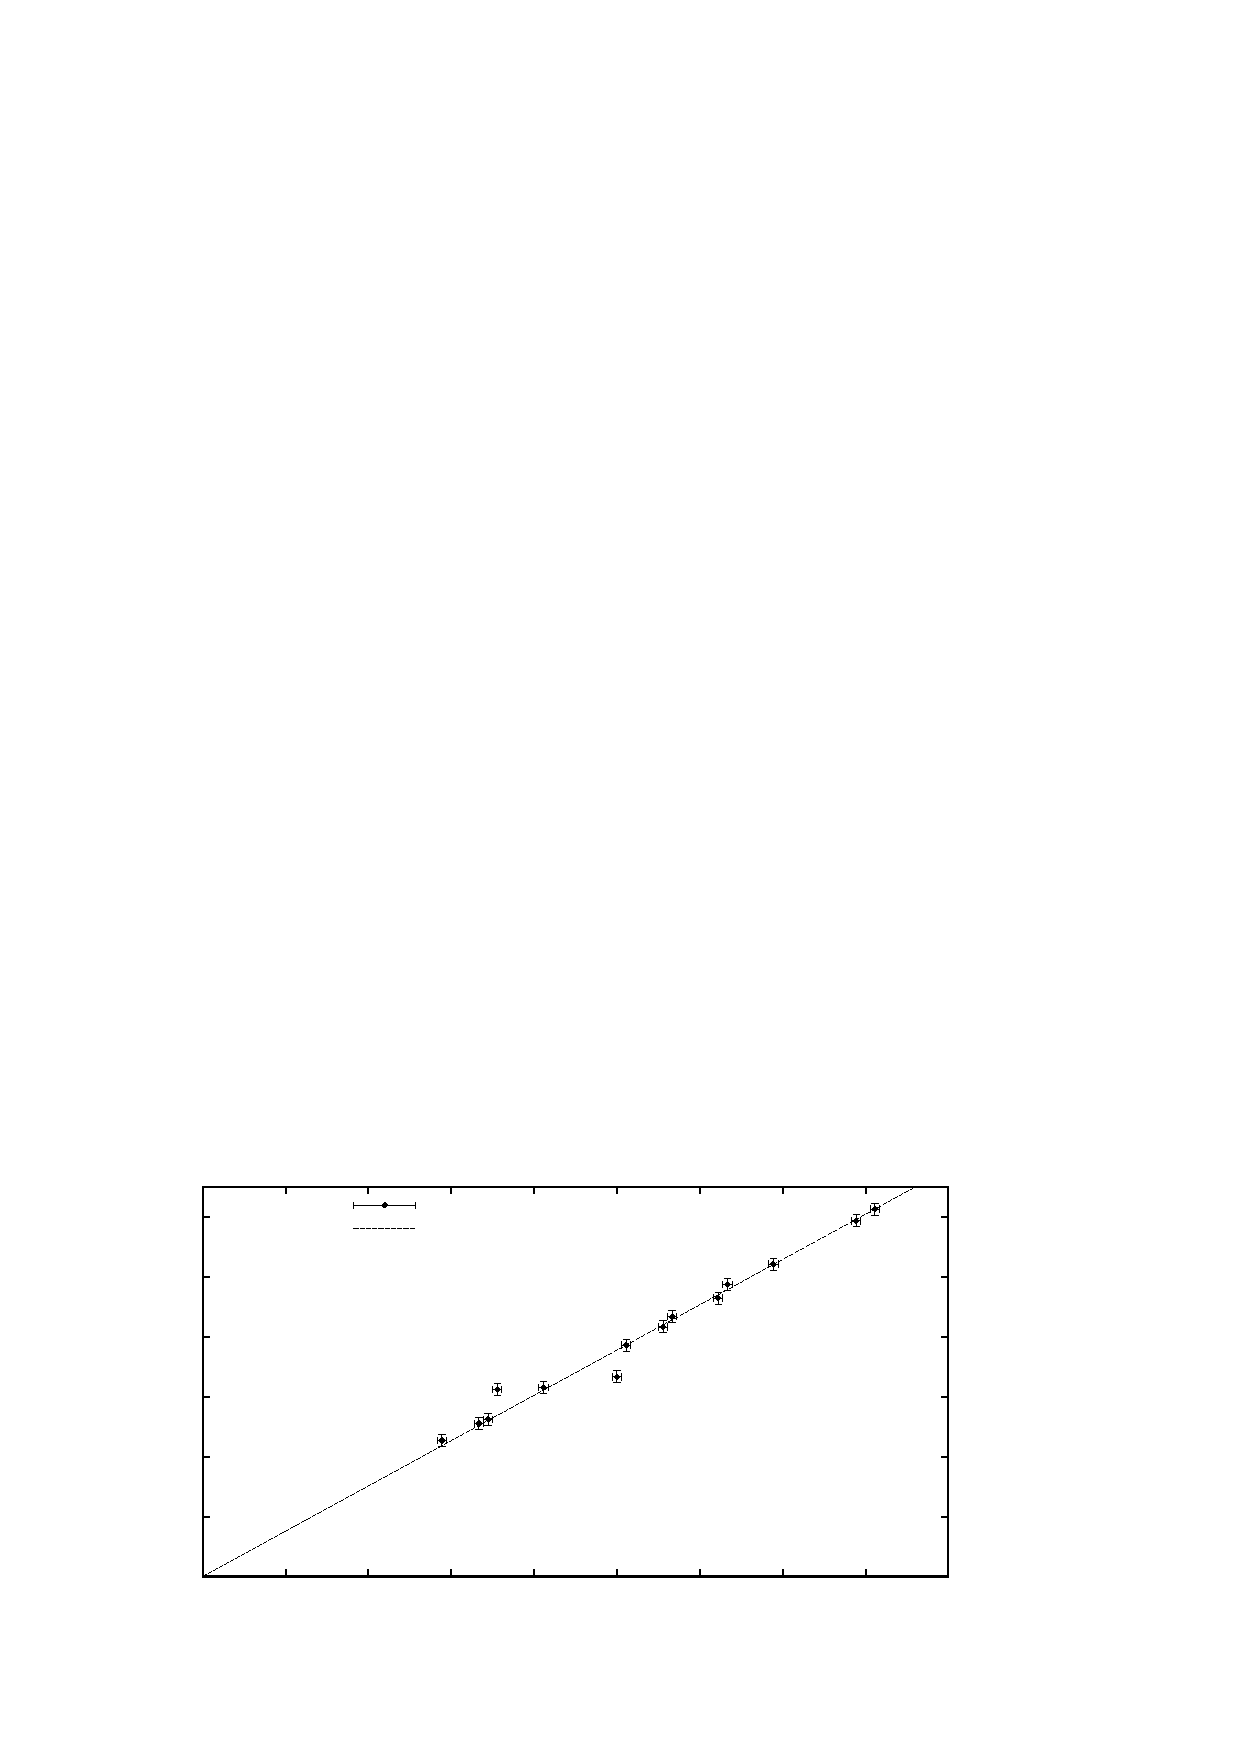
\includegraphics{nutation}}%
    \gplfronttext
  \end{picture}%
\endgroup

	\end{figure}

	\begin{figure}[h]
		\center
		% GNUPLOT: LaTeX picture with Postscript
\begingroup
  \makeatletter
  \providecommand\color[2][]{%
    \GenericError{(gnuplot) \space\space\space\@spaces}{%
      Package color not loaded in conjunction with
      terminal option `colourtext'%
    }{See the gnuplot documentation for explanation.%
    }{Either use 'blacktext' in gnuplot or load the package
      color.sty in LaTeX.}%
    \renewcommand\color[2][]{}%
  }%
  \providecommand\includegraphics[2][]{%
    \GenericError{(gnuplot) \space\space\space\@spaces}{%
      Package graphicx or graphics not loaded%
    }{See the gnuplot documentation for explanation.%
    }{The gnuplot epslatex terminal needs graphicx.sty or graphics.sty.}%
    \renewcommand\includegraphics[2][]{}%
  }%
  \providecommand\rotatebox[2]{#2}%
  \@ifundefined{ifGPcolor}{%
    \newif\ifGPcolor
    \GPcolorfalse
  }{}%
  \@ifundefined{ifGPblacktext}{%
    \newif\ifGPblacktext
    \GPblacktexttrue
  }{}%
  % define a \g@addto@macro without @ in the name:
  \let\gplgaddtomacro\g@addto@macro
  % define empty templates for all commands taking text:
  \gdef\gplbacktext{}%
  \gdef\gplfronttext{}%
  \makeatother
  \ifGPblacktext
    % no textcolor at all
    \def\colorrgb#1{}%
    \def\colorgray#1{}%
  \else
    % gray or color?
    \ifGPcolor
      \def\colorrgb#1{\color[rgb]{#1}}%
      \def\colorgray#1{\color[gray]{#1}}%
      \expandafter\def\csname LTw\endcsname{\color{white}}%
      \expandafter\def\csname LTb\endcsname{\color{black}}%
      \expandafter\def\csname LTa\endcsname{\color{black}}%
      \expandafter\def\csname LT0\endcsname{\color[rgb]{1,0,0}}%
      \expandafter\def\csname LT1\endcsname{\color[rgb]{0,1,0}}%
      \expandafter\def\csname LT2\endcsname{\color[rgb]{0,0,1}}%
      \expandafter\def\csname LT3\endcsname{\color[rgb]{1,0,1}}%
      \expandafter\def\csname LT4\endcsname{\color[rgb]{0,1,1}}%
      \expandafter\def\csname LT5\endcsname{\color[rgb]{1,1,0}}%
      \expandafter\def\csname LT6\endcsname{\color[rgb]{0,0,0}}%
      \expandafter\def\csname LT7\endcsname{\color[rgb]{1,0.3,0}}%
      \expandafter\def\csname LT8\endcsname{\color[rgb]{0.5,0.5,0.5}}%
    \else
      % gray
      \def\colorrgb#1{\color{black}}%
      \def\colorgray#1{\color[gray]{#1}}%
      \expandafter\def\csname LTw\endcsname{\color{white}}%
      \expandafter\def\csname LTb\endcsname{\color{black}}%
      \expandafter\def\csname LTa\endcsname{\color{black}}%
      \expandafter\def\csname LT0\endcsname{\color{black}}%
      \expandafter\def\csname LT1\endcsname{\color{black}}%
      \expandafter\def\csname LT2\endcsname{\color{black}}%
      \expandafter\def\csname LT3\endcsname{\color{black}}%
      \expandafter\def\csname LT4\endcsname{\color{black}}%
      \expandafter\def\csname LT5\endcsname{\color{black}}%
      \expandafter\def\csname LT6\endcsname{\color{black}}%
      \expandafter\def\csname LT7\endcsname{\color{black}}%
      \expandafter\def\csname LT8\endcsname{\color{black}}%
    \fi
  \fi
  \setlength{\unitlength}{0.0500bp}%
  \begin{picture}(8502.00,5102.00)%
    \gplgaddtomacro\gplbacktext{%
      \csname LTb\endcsname%
      \put(814,704){\makebox(0,0)[r]{\strut{}-50}}%
      \put(814,1451){\makebox(0,0)[r]{\strut{}-40}}%
      \put(814,2199){\makebox(0,0)[r]{\strut{}-30}}%
      \put(814,2946){\makebox(0,0)[r]{\strut{}-20}}%
      \put(814,3694){\makebox(0,0)[r]{\strut{}-10}}%
      \put(814,4441){\makebox(0,0)[r]{\strut{}0}}%
      \put(946,484){\makebox(0,0){\strut{}0.0}}%
      \put(1999,484){\makebox(0,0){\strut{}0.5}}%
      \put(3052,484){\makebox(0,0){\strut{}1.0}}%
      \put(4104,484){\makebox(0,0){\strut{}1.5}}%
      \put(5157,484){\makebox(0,0){\strut{}2.0}}%
      \put(6210,484){\makebox(0,0){\strut{}2.5}}%
      \put(7263,484){\makebox(0,0){\strut{}3.0}}%
      \put(176,2572){\rotatebox{-270}{\makebox(0,0){\strut{}$T_p \ [s]$}}}%
      \put(4525,154){\makebox(0,0){\strut{}$f_K \ [Hz]$}}%
      \put(4525,4771){\makebox(0,0){\strut{}$T_p(f_K)$ für verschiedene Abstände $s$}}%
      \put(1472,1451){\makebox(0,0)[l]{\strut{}$a \pm \Delta a = (-8.1693 \pm 0.1495) \ s^2$}}%
      \put(1472,1825){\makebox(0,0)[l]{\strut{}$b \pm \Delta b = (-15.662 \pm 0.340) \ s^2$}}%
    }%
    \gplgaddtomacro\gplfronttext{%
      \csname LTb\endcsname%
      \put(7118,4268){\makebox(0,0)[r]{\strut{}Messwerte $s = -20 \ mm$}}%
      \csname LTb\endcsname%
      \put(7118,4048){\makebox(0,0)[r]{\strut{}Messwerte $s = -10 \ mm$}}%
      \csname LTb\endcsname%
      \put(7118,3828){\makebox(0,0)[r]{\strut{}$f(x) = ax$}}%
      \csname LTb\endcsname%
      \put(7118,3608){\makebox(0,0)[r]{\strut{}$g(x) = bx$}}%
    }%
    \gplbacktext
    \put(0,0){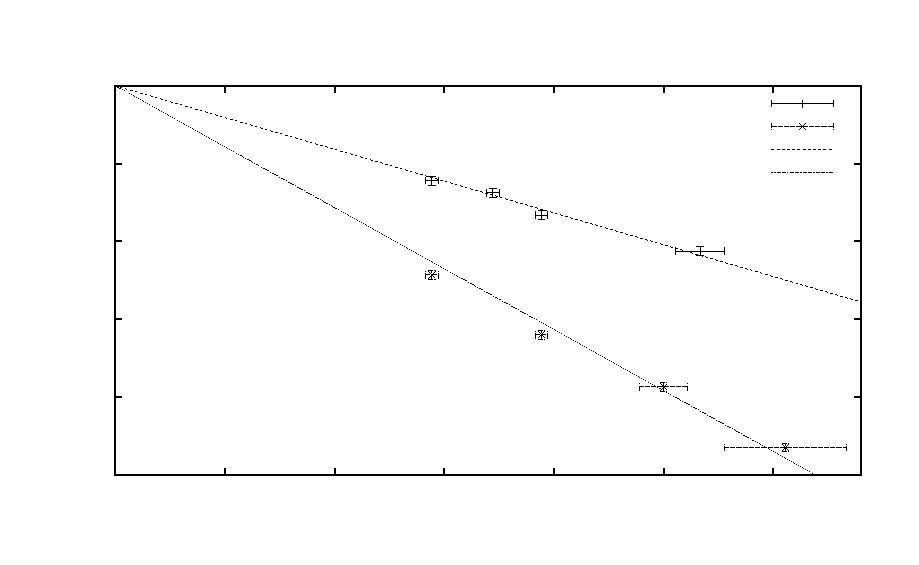
\includegraphics{praezession}}%
    \gplfronttext
  \end{picture}%
\endgroup

	\end{figure}

	\begin{figure}[h]
		\center
		% GNUPLOT: LaTeX picture with Postscript
\begingroup
  \makeatletter
  \providecommand\color[2][]{%
    \GenericError{(gnuplot) \space\space\space\@spaces}{%
      Package color not loaded in conjunction with
      terminal option `colourtext'%
    }{See the gnuplot documentation for explanation.%
    }{Either use 'blacktext' in gnuplot or load the package
      color.sty in LaTeX.}%
    \renewcommand\color[2][]{}%
  }%
  \providecommand\includegraphics[2][]{%
    \GenericError{(gnuplot) \space\space\space\@spaces}{%
      Package graphicx or graphics not loaded%
    }{See the gnuplot documentation for explanation.%
    }{The gnuplot epslatex terminal needs graphicx.sty or graphics.sty.}%
    \renewcommand\includegraphics[2][]{}%
  }%
  \providecommand\rotatebox[2]{#2}%
  \@ifundefined{ifGPcolor}{%
    \newif\ifGPcolor
    \GPcolorfalse
  }{}%
  \@ifundefined{ifGPblacktext}{%
    \newif\ifGPblacktext
    \GPblacktexttrue
  }{}%
  % define a \g@addto@macro without @ in the name:
  \let\gplgaddtomacro\g@addto@macro
  % define empty templates for all commands taking text:
  \gdef\gplbacktext{}%
  \gdef\gplfronttext{}%
  \makeatother
  \ifGPblacktext
    % no textcolor at all
    \def\colorrgb#1{}%
    \def\colorgray#1{}%
  \else
    % gray or color?
    \ifGPcolor
      \def\colorrgb#1{\color[rgb]{#1}}%
      \def\colorgray#1{\color[gray]{#1}}%
      \expandafter\def\csname LTw\endcsname{\color{white}}%
      \expandafter\def\csname LTb\endcsname{\color{black}}%
      \expandafter\def\csname LTa\endcsname{\color{black}}%
      \expandafter\def\csname LT0\endcsname{\color[rgb]{1,0,0}}%
      \expandafter\def\csname LT1\endcsname{\color[rgb]{0,1,0}}%
      \expandafter\def\csname LT2\endcsname{\color[rgb]{0,0,1}}%
      \expandafter\def\csname LT3\endcsname{\color[rgb]{1,0,1}}%
      \expandafter\def\csname LT4\endcsname{\color[rgb]{0,1,1}}%
      \expandafter\def\csname LT5\endcsname{\color[rgb]{1,1,0}}%
      \expandafter\def\csname LT6\endcsname{\color[rgb]{0,0,0}}%
      \expandafter\def\csname LT7\endcsname{\color[rgb]{1,0.3,0}}%
      \expandafter\def\csname LT8\endcsname{\color[rgb]{0.5,0.5,0.5}}%
    \else
      % gray
      \def\colorrgb#1{\color{black}}%
      \def\colorgray#1{\color[gray]{#1}}%
      \expandafter\def\csname LTw\endcsname{\color{white}}%
      \expandafter\def\csname LTb\endcsname{\color{black}}%
      \expandafter\def\csname LTa\endcsname{\color{black}}%
      \expandafter\def\csname LT0\endcsname{\color{black}}%
      \expandafter\def\csname LT1\endcsname{\color{black}}%
      \expandafter\def\csname LT2\endcsname{\color{black}}%
      \expandafter\def\csname LT3\endcsname{\color{black}}%
      \expandafter\def\csname LT4\endcsname{\color{black}}%
      \expandafter\def\csname LT5\endcsname{\color{black}}%
      \expandafter\def\csname LT6\endcsname{\color{black}}%
      \expandafter\def\csname LT7\endcsname{\color{black}}%
      \expandafter\def\csname LT8\endcsname{\color{black}}%
    \fi
  \fi
  \setlength{\unitlength}{0.0500bp}%
  \begin{picture}(8502.00,5102.00)%
    \gplgaddtomacro\gplbacktext{%
      \csname LTb\endcsname%
      \put(682,704){\makebox(0,0)[r]{\strut{}0}}%
      \put(682,1383){\makebox(0,0)[r]{\strut{}10}}%
      \put(682,2063){\makebox(0,0)[r]{\strut{}20}}%
      \put(682,2742){\makebox(0,0)[r]{\strut{}30}}%
      \put(682,3422){\makebox(0,0)[r]{\strut{}40}}%
      \put(682,4101){\makebox(0,0)[r]{\strut{}50}}%
      \put(814,484){\makebox(0,0){\strut{}0.0}}%
      \put(1682,484){\makebox(0,0){\strut{}0.5}}%
      \put(2550,484){\makebox(0,0){\strut{}1.0}}%
      \put(3418,484){\makebox(0,0){\strut{}1.5}}%
      \put(4286,484){\makebox(0,0){\strut{}2.0}}%
      \put(5154,484){\makebox(0,0){\strut{}2.5}}%
      \put(6022,484){\makebox(0,0){\strut{}3.0}}%
      \put(6890,484){\makebox(0,0){\strut{}3.5}}%
      \put(7758,484){\makebox(0,0){\strut{}4.0}}%
      \put(176,2572){\rotatebox{-270}{\makebox(0,0){\strut{}$T_p \ [s]$}}}%
      \put(4459,154){\makebox(0,0){\strut{}$f_K \ [Hz]$}}%
      \put(4459,4771){\makebox(0,0){\strut{}$T_p(f_K)$ für verschiedene Abstände $s$}}%
      \put(4980,1587){\makebox(0,0)[l]{\strut{}$a \pm \Delta a = (17.9941 \pm 0.3682) \ s^2$}}%
      \put(4980,1248){\makebox(0,0)[l]{\strut{}$b \pm \Delta b = (8.638 \pm 0.114) \ s^2$}}%
    }%
    \gplgaddtomacro\gplfronttext{%
      \csname LTb\endcsname%
      \put(3718,4268){\makebox(0,0)[r]{\strut{}Messwerte $s = 10 \ mm$}}%
      \csname LTb\endcsname%
      \put(3718,4048){\makebox(0,0)[r]{\strut{}Messwerte $s = 20 \ mm$}}%
      \csname LTb\endcsname%
      \put(3718,3828){\makebox(0,0)[r]{\strut{}$f(x) = ax$}}%
      \csname LTb\endcsname%
      \put(3718,3608){\makebox(0,0)[r]{\strut{}$g(x) = bx$}}%
    }%
    \gplbacktext
    \put(0,0){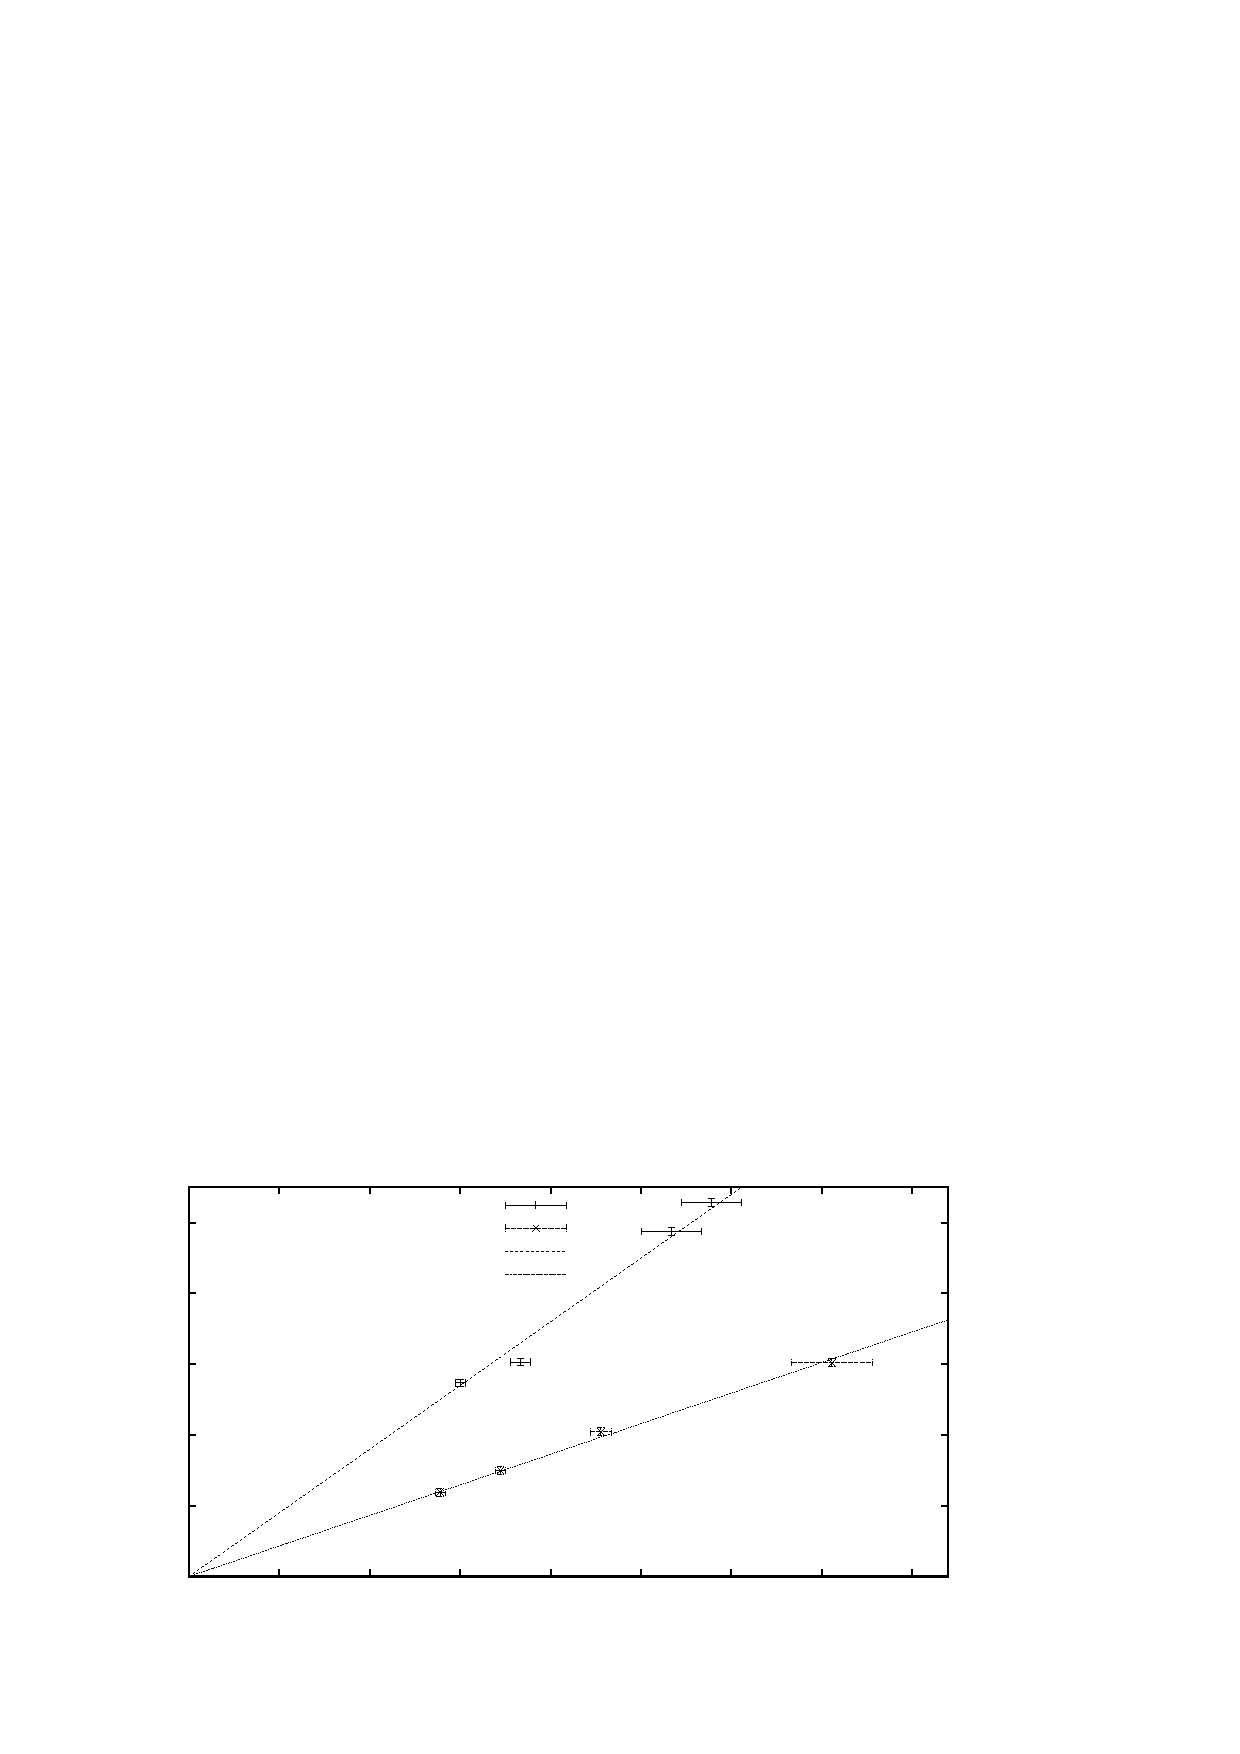
\includegraphics{praezession2}}%
    \gplfronttext
  \end{picture}%
\endgroup

	\end{figure}

	\begin{figure}[h]
		\center
		% GNUPLOT: LaTeX picture with Postscript
\begingroup
  \makeatletter
  \providecommand\color[2][]{%
    \GenericError{(gnuplot) \space\space\space\@spaces}{%
      Package color not loaded in conjunction with
      terminal option `colourtext'%
    }{See the gnuplot documentation for explanation.%
    }{Either use 'blacktext' in gnuplot or load the package
      color.sty in LaTeX.}%
    \renewcommand\color[2][]{}%
  }%
  \providecommand\includegraphics[2][]{%
    \GenericError{(gnuplot) \space\space\space\@spaces}{%
      Package graphicx or graphics not loaded%
    }{See the gnuplot documentation for explanation.%
    }{The gnuplot epslatex terminal needs graphicx.sty or graphics.sty.}%
    \renewcommand\includegraphics[2][]{}%
  }%
  \providecommand\rotatebox[2]{#2}%
  \@ifundefined{ifGPcolor}{%
    \newif\ifGPcolor
    \GPcolorfalse
  }{}%
  \@ifundefined{ifGPblacktext}{%
    \newif\ifGPblacktext
    \GPblacktexttrue
  }{}%
  % define a \g@addto@macro without @ in the name:
  \let\gplgaddtomacro\g@addto@macro
  % define empty templates for all commands taking text:
  \gdef\gplbacktext{}%
  \gdef\gplfronttext{}%
  \makeatother
  \ifGPblacktext
    % no textcolor at all
    \def\colorrgb#1{}%
    \def\colorgray#1{}%
  \else
    % gray or color?
    \ifGPcolor
      \def\colorrgb#1{\color[rgb]{#1}}%
      \def\colorgray#1{\color[gray]{#1}}%
      \expandafter\def\csname LTw\endcsname{\color{white}}%
      \expandafter\def\csname LTb\endcsname{\color{black}}%
      \expandafter\def\csname LTa\endcsname{\color{black}}%
      \expandafter\def\csname LT0\endcsname{\color[rgb]{1,0,0}}%
      \expandafter\def\csname LT1\endcsname{\color[rgb]{0,1,0}}%
      \expandafter\def\csname LT2\endcsname{\color[rgb]{0,0,1}}%
      \expandafter\def\csname LT3\endcsname{\color[rgb]{1,0,1}}%
      \expandafter\def\csname LT4\endcsname{\color[rgb]{0,1,1}}%
      \expandafter\def\csname LT5\endcsname{\color[rgb]{1,1,0}}%
      \expandafter\def\csname LT6\endcsname{\color[rgb]{0,0,0}}%
      \expandafter\def\csname LT7\endcsname{\color[rgb]{1,0.3,0}}%
      \expandafter\def\csname LT8\endcsname{\color[rgb]{0.5,0.5,0.5}}%
    \else
      % gray
      \def\colorrgb#1{\color{black}}%
      \def\colorgray#1{\color[gray]{#1}}%
      \expandafter\def\csname LTw\endcsname{\color{white}}%
      \expandafter\def\csname LTb\endcsname{\color{black}}%
      \expandafter\def\csname LTa\endcsname{\color{black}}%
      \expandafter\def\csname LT0\endcsname{\color{black}}%
      \expandafter\def\csname LT1\endcsname{\color{black}}%
      \expandafter\def\csname LT2\endcsname{\color{black}}%
      \expandafter\def\csname LT3\endcsname{\color{black}}%
      \expandafter\def\csname LT4\endcsname{\color{black}}%
      \expandafter\def\csname LT5\endcsname{\color{black}}%
      \expandafter\def\csname LT6\endcsname{\color{black}}%
      \expandafter\def\csname LT7\endcsname{\color{black}}%
      \expandafter\def\csname LT8\endcsname{\color{black}}%
    \fi
  \fi
  \setlength{\unitlength}{0.0500bp}%
  \begin{picture}(8502.00,5102.00)%
    \gplgaddtomacro\gplbacktext{%
      \csname LTb\endcsname%
      \put(814,704){\makebox(0,0)[r]{\strut{}-20}}%
      \put(814,1171){\makebox(0,0)[r]{\strut{}-15}}%
      \put(814,1638){\makebox(0,0)[r]{\strut{}-10}}%
      \put(814,2105){\makebox(0,0)[r]{\strut{}-5}}%
      \put(814,2573){\makebox(0,0)[r]{\strut{}0}}%
      \put(814,3040){\makebox(0,0)[r]{\strut{}5}}%
      \put(814,3507){\makebox(0,0)[r]{\strut{}10}}%
      \put(814,3974){\makebox(0,0)[r]{\strut{}15}}%
      \put(814,4441){\makebox(0,0)[r]{\strut{}20}}%
      \put(946,484){\makebox(0,0){\strut{}-0.15}}%
      \put(2139,484){\makebox(0,0){\strut{}-0.10}}%
      \put(3332,484){\makebox(0,0){\strut{}-0.05}}%
      \put(4526,484){\makebox(0,0){\strut{}0.00}}%
      \put(5719,484){\makebox(0,0){\strut{}0.05}}%
      \put(6912,484){\makebox(0,0){\strut{}0.10}}%
      \put(8105,484){\makebox(0,0){\strut{}0.15}}%
      \put(176,2572){\rotatebox{-270}{\makebox(0,0){\strut{}$T_p/f_K \ [s^2]$}}}%
      \put(4525,154){\makebox(0,0){\strut{}$1/s \ [mm^{-1}]$}}%
      \put(4525,4771){\makebox(0,0){\strut{}$T_p/f_K$ über $1/s$}}%
      \put(1423,3507){\makebox(0,0)[l]{\strut{}$ a \pm \Delta a = (166.05 \pm 0.67) \ mm \cdot s^2$}}%
    }%
    \gplgaddtomacro\gplfronttext{%
      \csname LTb\endcsname%
      \put(2266,4268){\makebox(0,0)[r]{\strut{}Messwerte}}%
      \csname LTb\endcsname%
      \put(2266,4048){\makebox(0,0)[r]{\strut{}$f(x) = ax$}}%
    }%
    \gplbacktext
    \put(0,0){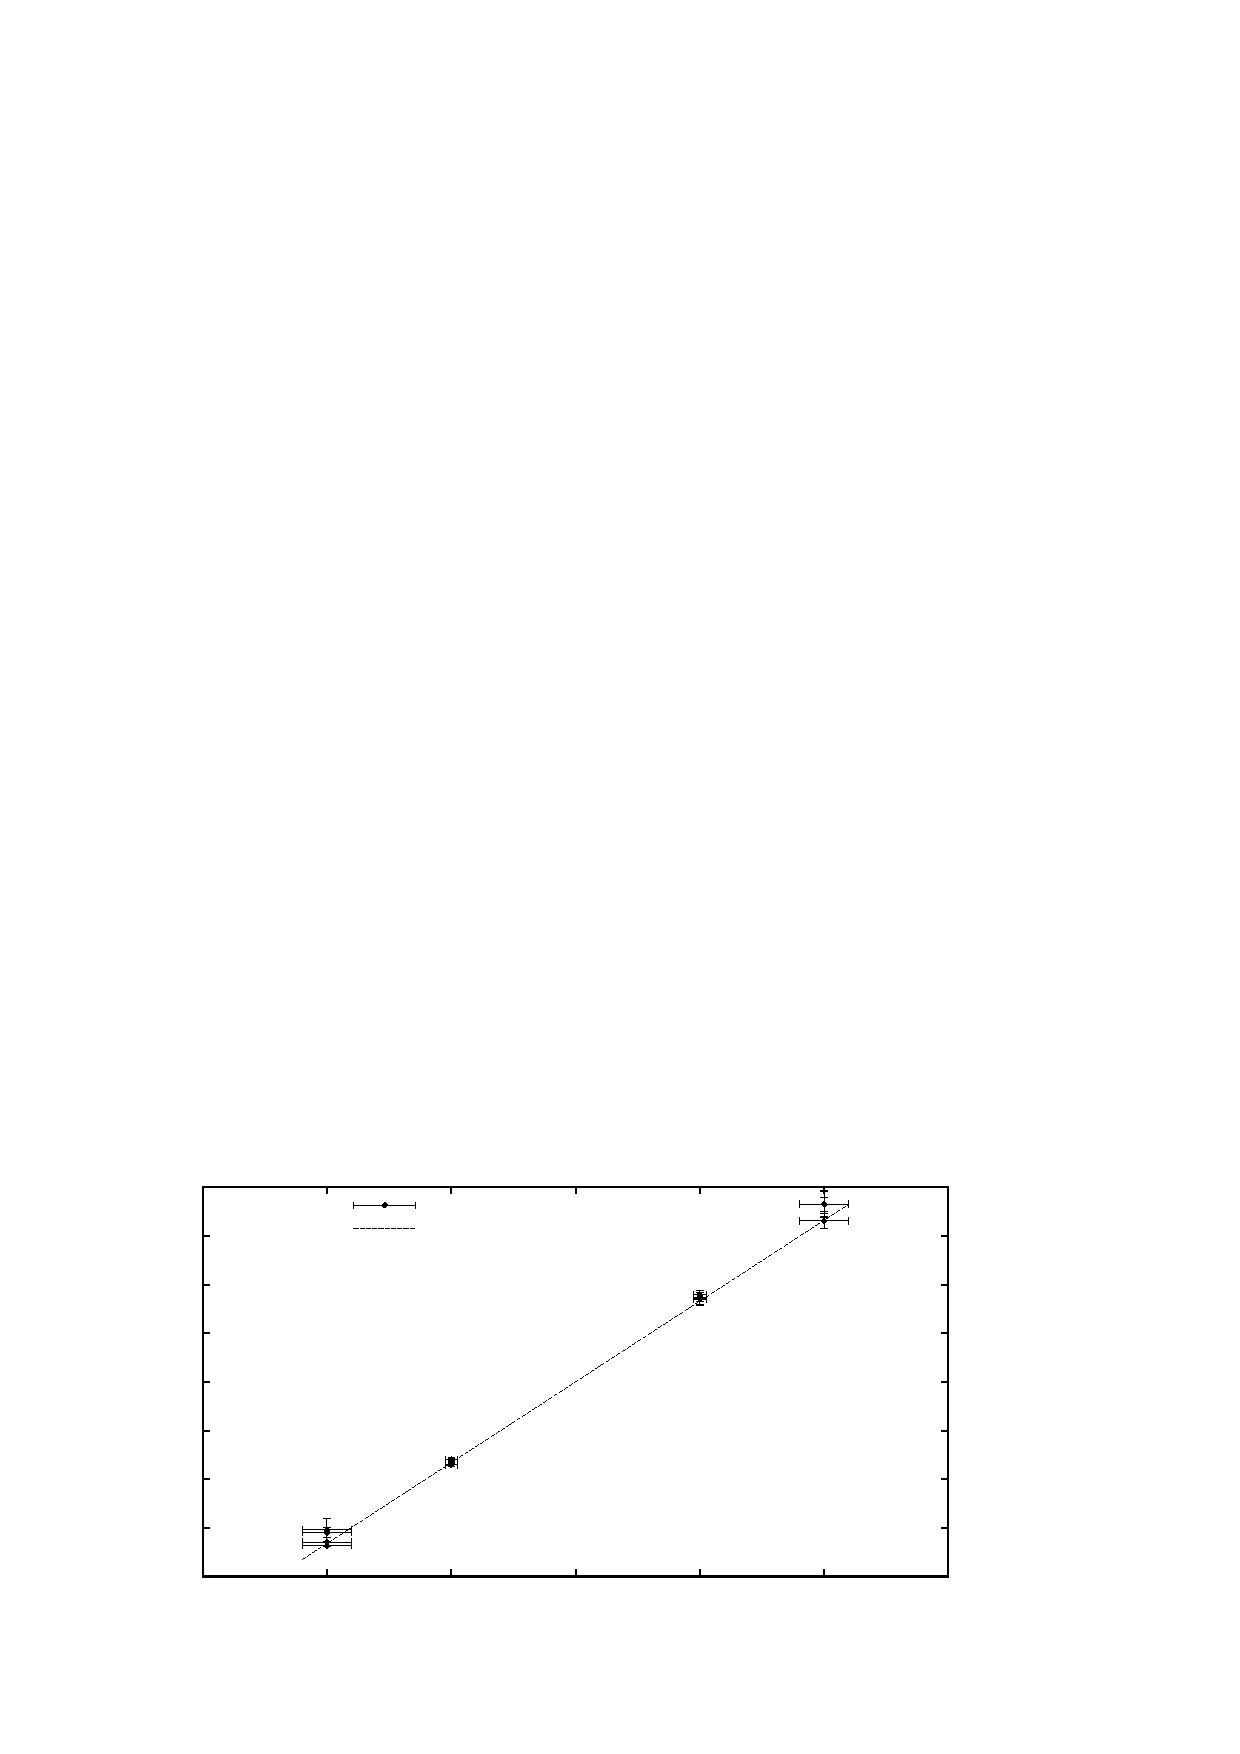
\includegraphics{praezession3}}%
    \gplfronttext
  \end{picture}%
\endgroup

	\end{figure}

	\begin{figure}[h]
		\center
		% GNUPLOT: LaTeX picture with Postscript
\begingroup
  \makeatletter
  \providecommand\color[2][]{%
    \GenericError{(gnuplot) \space\space\space\@spaces}{%
      Package color not loaded in conjunction with
      terminal option `colourtext'%
    }{See the gnuplot documentation for explanation.%
    }{Either use 'blacktext' in gnuplot or load the package
      color.sty in LaTeX.}%
    \renewcommand\color[2][]{}%
  }%
  \providecommand\includegraphics[2][]{%
    \GenericError{(gnuplot) \space\space\space\@spaces}{%
      Package graphicx or graphics not loaded%
    }{See the gnuplot documentation for explanation.%
    }{The gnuplot epslatex terminal needs graphicx.sty or graphics.sty.}%
    \renewcommand\includegraphics[2][]{}%
  }%
  \providecommand\rotatebox[2]{#2}%
  \@ifundefined{ifGPcolor}{%
    \newif\ifGPcolor
    \GPcolorfalse
  }{}%
  \@ifundefined{ifGPblacktext}{%
    \newif\ifGPblacktext
    \GPblacktexttrue
  }{}%
  % define a \g@addto@macro without @ in the name:
  \let\gplgaddtomacro\g@addto@macro
  % define empty templates for all commands taking text:
  \gdef\gplbacktext{}%
  \gdef\gplfronttext{}%
  \makeatother
  \ifGPblacktext
    % no textcolor at all
    \def\colorrgb#1{}%
    \def\colorgray#1{}%
  \else
    % gray or color?
    \ifGPcolor
      \def\colorrgb#1{\color[rgb]{#1}}%
      \def\colorgray#1{\color[gray]{#1}}%
      \expandafter\def\csname LTw\endcsname{\color{white}}%
      \expandafter\def\csname LTb\endcsname{\color{black}}%
      \expandafter\def\csname LTa\endcsname{\color{black}}%
      \expandafter\def\csname LT0\endcsname{\color[rgb]{1,0,0}}%
      \expandafter\def\csname LT1\endcsname{\color[rgb]{0,1,0}}%
      \expandafter\def\csname LT2\endcsname{\color[rgb]{0,0,1}}%
      \expandafter\def\csname LT3\endcsname{\color[rgb]{1,0,1}}%
      \expandafter\def\csname LT4\endcsname{\color[rgb]{0,1,1}}%
      \expandafter\def\csname LT5\endcsname{\color[rgb]{1,1,0}}%
      \expandafter\def\csname LT6\endcsname{\color[rgb]{0,0,0}}%
      \expandafter\def\csname LT7\endcsname{\color[rgb]{1,0.3,0}}%
      \expandafter\def\csname LT8\endcsname{\color[rgb]{0.5,0.5,0.5}}%
    \else
      % gray
      \def\colorrgb#1{\color{black}}%
      \def\colorgray#1{\color[gray]{#1}}%
      \expandafter\def\csname LTw\endcsname{\color{white}}%
      \expandafter\def\csname LTb\endcsname{\color{black}}%
      \expandafter\def\csname LTa\endcsname{\color{black}}%
      \expandafter\def\csname LT0\endcsname{\color{black}}%
      \expandafter\def\csname LT1\endcsname{\color{black}}%
      \expandafter\def\csname LT2\endcsname{\color{black}}%
      \expandafter\def\csname LT3\endcsname{\color{black}}%
      \expandafter\def\csname LT4\endcsname{\color{black}}%
      \expandafter\def\csname LT5\endcsname{\color{black}}%
      \expandafter\def\csname LT6\endcsname{\color{black}}%
      \expandafter\def\csname LT7\endcsname{\color{black}}%
      \expandafter\def\csname LT8\endcsname{\color{black}}%
    \fi
  \fi
  \setlength{\unitlength}{0.0500bp}%
  \begin{picture}(8502.00,5102.00)%
    \gplgaddtomacro\gplbacktext{%
      \csname LTb\endcsname%
      \put(814,704){\makebox(0,0)[r]{\strut{} 0}}%
      \put(814,1553){\makebox(0,0)[r]{\strut{} 5}}%
      \put(814,2403){\makebox(0,0)[r]{\strut{} 10}}%
      \put(814,3252){\makebox(0,0)[r]{\strut{} 15}}%
      \put(814,4101){\makebox(0,0)[r]{\strut{} 20}}%
      \put(946,484){\makebox(0,0){\strut{} 0}}%
      \put(2378,484){\makebox(0,0){\strut{} 0.05}}%
      \put(3810,484){\makebox(0,0){\strut{} 0.1}}%
      \put(5241,484){\makebox(0,0){\strut{} 0.15}}%
      \put(6673,484){\makebox(0,0){\strut{} 0.2}}%
      \put(8105,484){\makebox(0,0){\strut{} 0.25}}%
      \put(176,2572){\rotatebox{-270}{\makebox(0,0){\strut{}$T^2 \ [s^2]$}}}%
      \put(4525,154){\makebox(0,0){\strut{}$1/s \ [mm^{-1}]$}}%
      \put(4525,4771){\makebox(0,0){\strut{}Messwerte $T^2(1/s)$}}%
      \put(1519,3422){\makebox(0,0)[l]{\strut{}$ a\pm \Delta a = (103.0 \pm 3.3) \ mm \cdot s^2 $}}%
    }%
    \gplgaddtomacro\gplfronttext{%
      \csname LTb\endcsname%
      \put(2266,4268){\makebox(0,0)[r]{\strut{}Messwerte}}%
      \csname LTb\endcsname%
      \put(2266,4048){\makebox(0,0)[r]{\strut{}$f(x) = ax$}}%
    }%
    \gplbacktext
    \put(0,0){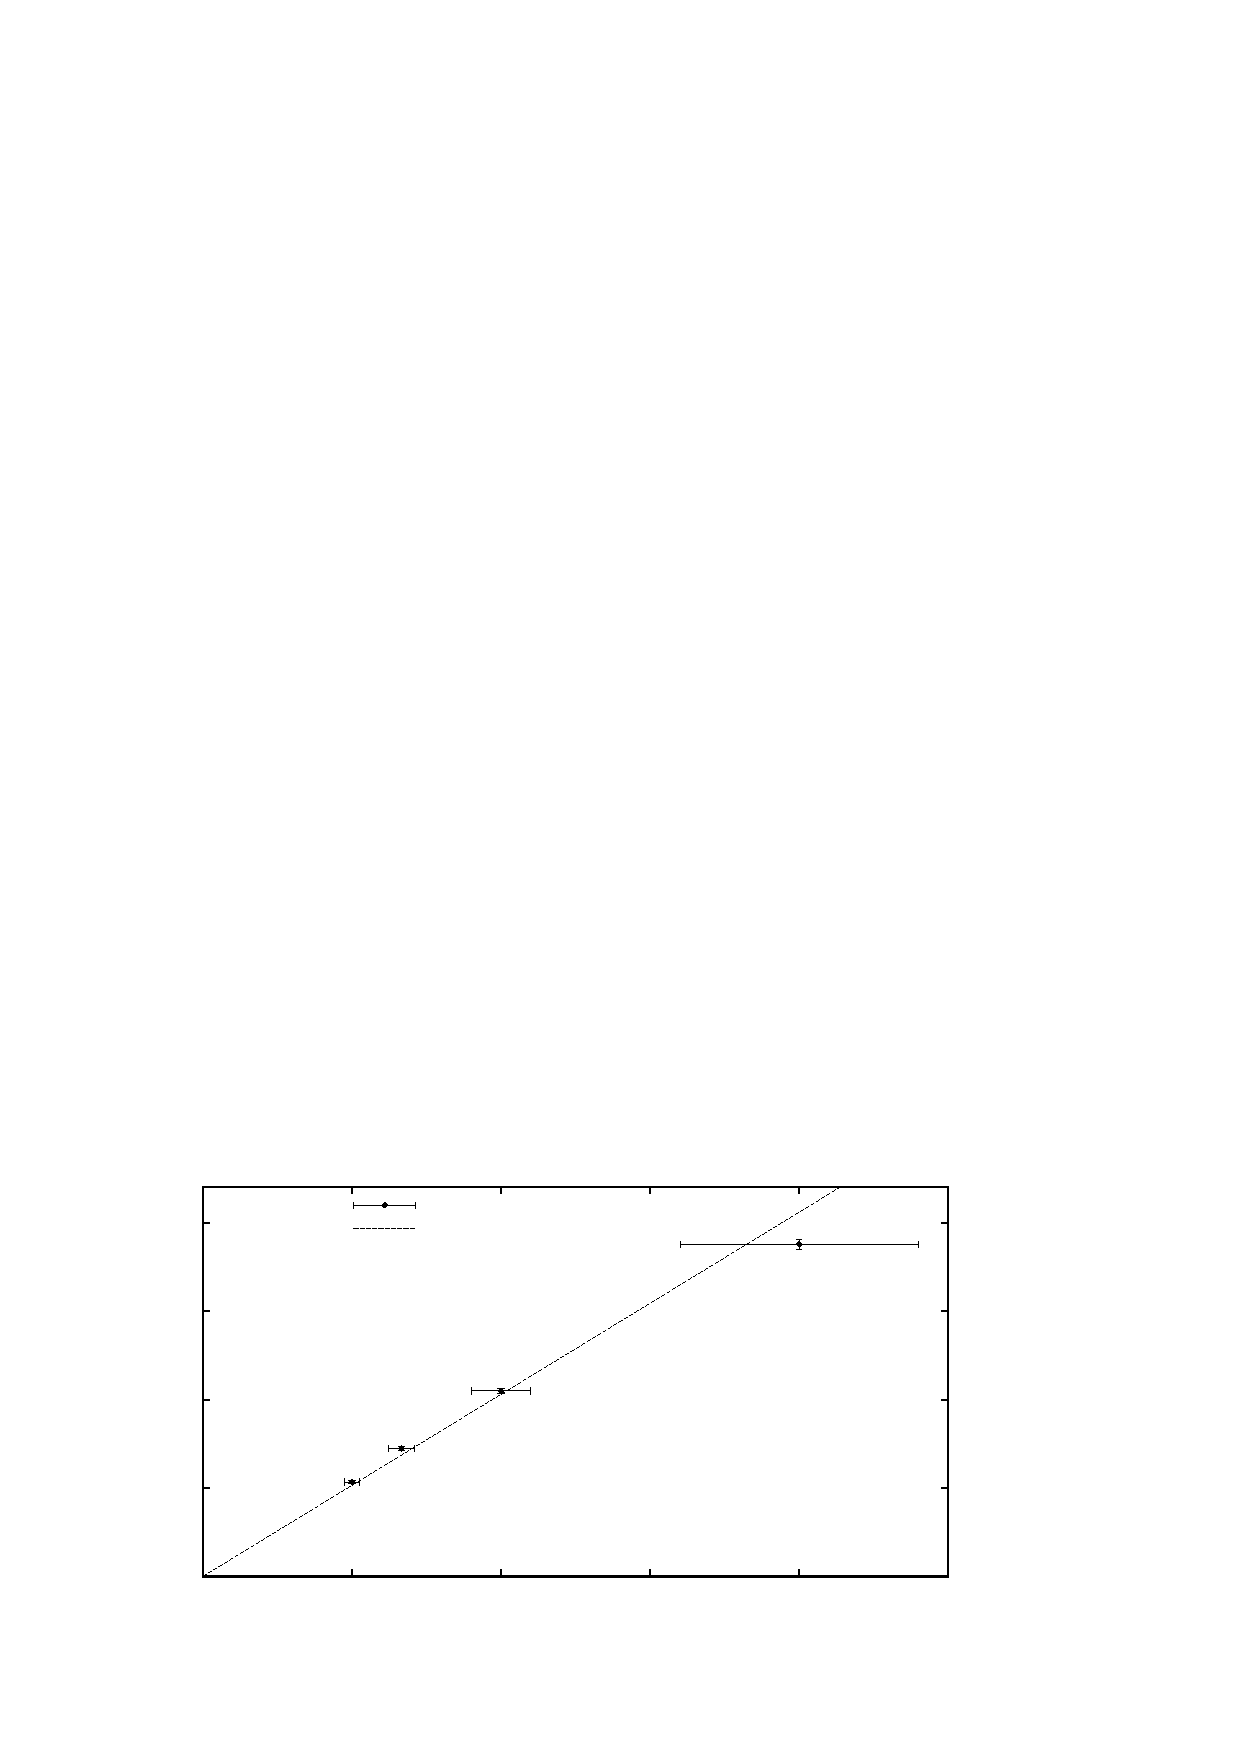
\includegraphics{js}}%
    \gplfronttext
  \end{picture}%
\endgroup

	\end{figure}

\end{document}

